% Created 2026-06-18 Thu 21:49
% Intended LaTeX compiler: pdflatex
\documentclass[presentation]{beamer}
\usepackage[utf8]{inputenc}
\usepackage[T1]{fontenc}
\usepackage{graphicx}
\usepackage{longtable}
\usepackage{wrapfig}
\usepackage{rotating}
\usepackage[normalem]{ulem}
\usepackage{amsmath}
\usepackage{amssymb}
\usepackage{capt-of}
\usepackage{hyperref}
\usepackage[T1]{fontenc}
\usepackage[utf8]{inputenc}
\usepackage[spanish]{babel}
\usepackage[backend=biber, style=apa]{biblatex}
\addbibresource{/home/arielmontufar/Exposicion/BusesDelSistema_G1-G2/bibliography/bibliography.bib}
\usetheme{default}
\usecolortheme{}
\usefonttheme{}
\useinnertheme{}
\useoutertheme{}
\author{Lenin G. Falconí}
\date{}
\title{S8 — Buses del Sistema}

\hypersetup{
 pdfauthor={Lenin G. Falconí},
 pdftitle={S8 — Buses del Sistema},
 pdfkeywords={},
 pdfsubject={},
 pdfcreator={Emacs 27.1 (Org mode 9.3)}, 
 pdflang={Spanish}}
\begin{document}

\maketitle
\begin{frame}{Outline}
\tableofcontents
\end{frame}


\section{Indicaciones}
\label{sec:org15bc2f6}
\begin{frame}[fragile,allowframebreaks]{Indicaciones}
 \begin{itemize}
\item Recuerde que si \texttt{options: H:2}, entonces:
\begin{itemize}
\item \texttt{*} Declara el nombre de la Sección
\item \texttt{**} Declara el nombre de la diapositiva
\end{itemize}
\item Puede alterar la estructura de la diapositiva si lo considera necesario
\item Reparto del tema por grupos:
\begin{itemize}
\item \alert{G1:} Estructuras de Interconexión, Interconexión punto a punto, QPI
\item \alert{G2:} Interconexión con Buses, Jerarquía de Buses, Elementos de Diseño, PCI Express
\end{itemize}
\item Para este tema consulte las siguientes fuentes:
\begin{itemize}
\item \textcite{stallings2006esp}, 7ma edición, 2006, Español, páginas 99 a 119.
\item \textcite{stallings2022computer}, 11ava edición, 2022, English, páginas 116 a 131.
\end{itemize}
\item Las tuplas (7, 99) significan: Edición 7, página 99 del PDF.
\item El grupo expone el tema y sube la presentación (\texttt{.ORG} y \texttt{.PDF} para Beamer, o \texttt{.ORG} y \texttt{.HTML} para reveal.js)
\item El grupo sube las ayudas memoria/notas del tema usando la plantilla \url{FormatoTareas/TemplateNotasClase.org} (\texttt{.ORG} y \texttt{.PDF})
\end{itemize}
\end{frame}
\begin{frame}[label={sec:orga9b299c},fragile]{Diseño de las Diapositivas}
 \begin{itemize}
\item Para diseñar sus diapositivas puede consultar cualquiera de las
presentaciones \texttt{.ORG} desarrolladas por el profesor así como al
archivo \href{https://github.com/LeninGF/EPN-Lectures/blob/main/iccd332ArqComp-2024-B/Tutoriales/Beamer-Emacs/tutorialBeamer.org}{tutorialBeamer.org} en el repositorio de la clase.
\item Recuerde que los archivos \texttt{.ORG} son archivos de texto así que los
puede copiar y sustituir por su texto propio.
\end{itemize}
\end{frame}
\begin{frame}[label={sec:orgb2b5550}]{Sobre este Documento}
\begin{itemize}
\item Este documento tiene la propuesta de temas a tratar y desarrollar
por los estudiantes.
\item Se ha de utilizar como base la bibliografía recomendada, pero puede
consultar bibliografía adicional.
\end{itemize}
\end{frame}
\section{Buses del Sistema}
\label{sec:org57abc5d}
\begin{frame}[label={sec:org4671a2b}]{Estructuras de Interconexión (7, 97)}
\end{frame}
\section{Interconexión con Buses}
\label{sec:orgf9ff483}
\begin{frame}[label={sec:org7eeca4a}]{Interconexión con Buses (7, 99)}
\end{frame}
\begin{frame}[label={sec:org6f6583d}]{Estructura del Bus  (7, 99)}
\end{frame}
\begin{frame}[label={sec:orga9b7937}]{Jerarquía de Buses Múltiples (7, 102)}
\end{frame}
\begin{frame}[label={sec:org05e0997}]{Elementos de Diseño de un Bus (7, 104)}
\end{frame}
\section{Interconexión punto a punto}
\label{sec:org2a181ad}
\begin{frame}[label={sec:orgd87d7d9}]{Problemas del bus compartido tradicional}
\begin{center}
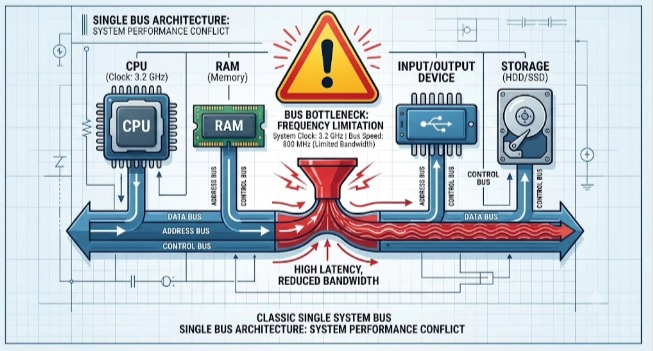
\includegraphics[width=.9\linewidth]{./images/BusCuelloDeBotella.jpeg}
\end{center}
-Restricciones eléctricas: Al subir la frecuencia del reloj para ganar velocidad, el bus tradicional falla\\[0pt]
-El problema: Con tasas de datos tan altas, es casi imposible realizar la sincronización y el arbitraje a tiempo y sin errores\\[0pt]
\end{frame}
\begin{frame}[label={sec:org9829613}]{El Reemplazo: Interconexión Punto a Punto}
\begin{center}
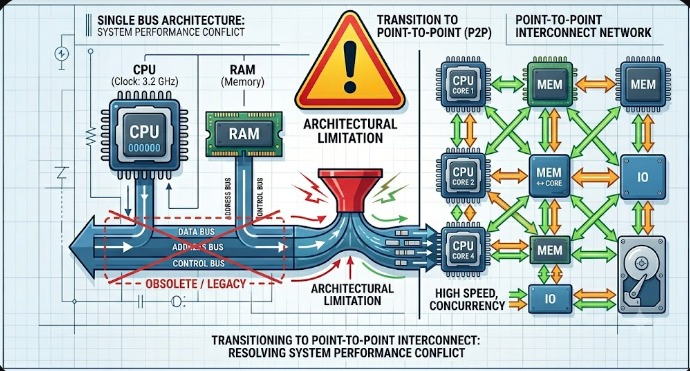
\includegraphics[width=.9\linewidth]{./images/InterconexionPuntoaPunto.jpeg}
\end{center}
-El nuevo estándar: El bus compartido ha sido reemplazado casi por completo por interconexiones punto a punto\\[0pt]
-Ventajas: Menos latencia, una tasa de datos significativamente más alta y mejor escalabilidad\\[0pt]
\end{frame}
\begin{frame}[label={sec:org8c436d1}]{El Reemplazo: Las 3 características modernas (Arquitectura)}
\begin{center}
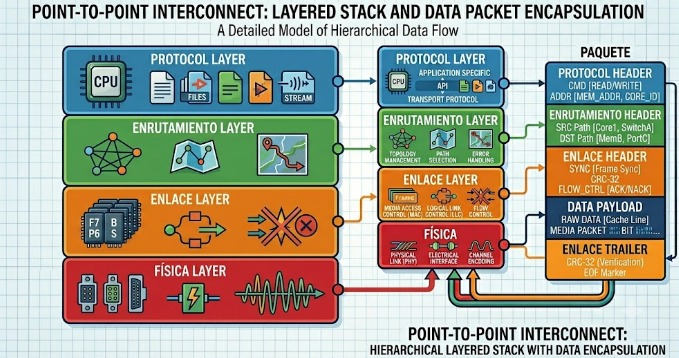
\includegraphics[width=.9\linewidth]{./images/CapasIPP.jpeg}
\end{center}
\begin{enumerate}
\item Conexiones directas por parejas: Al enlazar directamente dos componentes, se elimina por completo la necesidad de arbitraje
\item Arquitectura de protocolos en capas: Se estructuran de forma similar a las redes de datos (como TCP/IP)
\item Transferencia por paquetes: Los datos no fluyen crudos; se envían como secuencias de paquetes que incluyen cabeceras y detección de errores
\end{enumerate}
\end{frame}
\begin{frame}[label={sec:org60d5d96}]{QPI (11, 120)}
\end{frame}
\section{PCI Express}
\label{sec:org0de116d}
\begin{frame}[label={sec:org1ddc2e6}]{PCI Express (11, 123)}
\end{frame}
\section{Referencias}
\label{sec:org10c199f}
\begin{frame}[allowframebreaks]{Bibliografía}
\printbibliography
\end{frame}
\end{document}
